\section{Modulationsarten}
Modulationsverfahren sind ein großes Anwendungsgebiet in der Nachrichtentechnik.
Ziel ist es, viele Informationen verlustfrei zu übertragen.
Möchte man ein Datensignal übertragen, muss es davor
aufbereitet werden. Dies erledigt der Modulator/Mischer.
\\
Es gibt analoge und digitale Modulationsarten.
Es folgen einige Beispiele:


\subsection{Amplitudenmodulation}
\subsubsection{Analoge Amplitudenmodulation AM}
Die Idee hinter der Amplitudenmodulation ist, dass das Informationssignal
auf die Amplitude des Trägersignals moduliert wird.
Dadurch verändert sich die Amplitude des Trägersignals in Abhängigkeit vom Pegel und
der Frequenz des Informationssignals.
\begin{figure}[H]
    \centering
    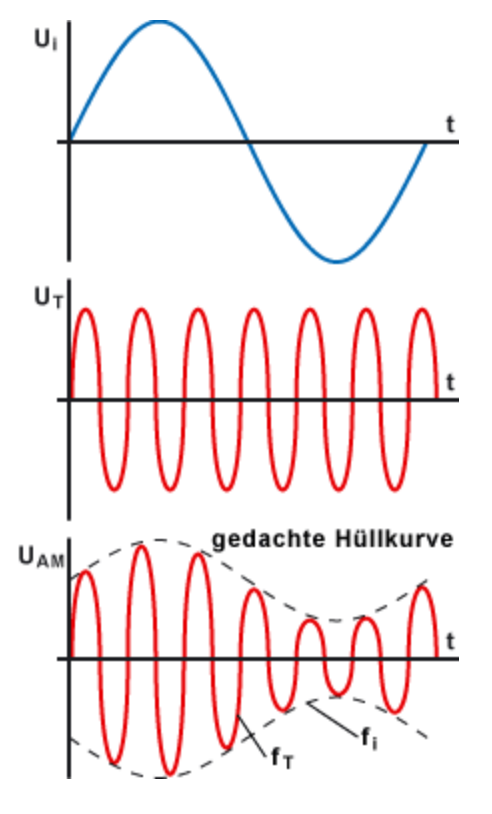
\includegraphics[width=0.20\textwidth]{Pictures/Screenshot 2025-06-19 125508.png}
    \caption{Amplitudenmodulation}
    \footnotesize{Quelle: \url{https://www.elektronik-kompendium.de/sites/kom/0401181.htm}}
    \label{fig:link_budget}
\end{figure}
Die Amplitude der Trägerschwingung wird durch das analoge Datensignal
$x(t)$ folgendermaßen verändert:
\begin{equation}
    a(t)=A_c(1+\mu x(t))
\end{equation}
Das AM-Signal wird beschrieben durch:
\begin{equation}
    x_c(t)=A_c(1+\mu x(t))cos(2\pi f_c t)
\end{equation}
\begin{itemize}
    \item $A_c$: Trägeramplitude
    \item $f_c$: Trägerfrequenz
    \item $\mu$: Modulationsindex $0 < \mu < 1$
\end{itemize}
\subsubsection{Digitale Amplitudenmodulation ASK}
Einer der einfachsten digitalen Modulationsverfahren ist 
das On-Off-Keying. 
Die Idee ist ganz simpel: Man hat ein digitales Datensignal aus Nullen und Einsen
und ein Sinus-/Kosinus-Signal von einem Oszillator, das als Trägerfrequenz fungiert.
Und je nachdem, ob eine Null oder Eins anliegt, wird dann der Oszillator angeschaltet bzw. ausgeschaltet.
Mathematisch ausgedrückt heißt das:
\begin{equation}
s(t) =
\begin{cases}
0, & \text{für Bit } = 0 \\
A \cdot \cos(2 \pi f_c t), & \text{für Bit } = 1
\end{cases}
\end{equation}




\subsection{Frequenzmodulation FM}
Die Frequenzmodulation spielt eine ebenso wichtige Rolle wie die Amplitudenmodulation,
ist im Vergleich jedoch weniger störanfällig. 
Hier wird auch ein hochfrequentes Trägersignal erzeugt und dadurch die Sendefrequenz um einen kleinen Betrag verändert.
Am einfachsten ist so eine Modulation durch einen LC-Schwingkreis.

\begin{equation}
x_c(t) = A_c \cos\left( 2\pi f_c t + 2\pi f_\Delta \int_0^t x(\tau) \, \mathrm{d}\tau \right)
\end{equation}
\begin{itemize}
    \item $x(\tau)$: Datensignal
    \item $A_c$: Amplitude des Trägersignals (konstant)
    \item $f_c$: Trägerfrequenz 
    \item $f_\Delta$: Frequenzhub, legt die maximale Abweichung zu $f_c$ fest
\end{itemize}
\clearpage

\subsection{Phasenmodulation PM}
Die Phasenmodulation gehört wie die Frequenzmodulation zu den Winkelmodulationen.
Hier wird die Phase der Trägerwelle in Abhängigkeit vom Datensignal verändert.
Die Phasenveränderung bleibt im Signal erhalten, variiert jedoch im Vergleich
zur ursprünglichen Phase des Trägersignals.
\begin{figure}[h]
    \centering
    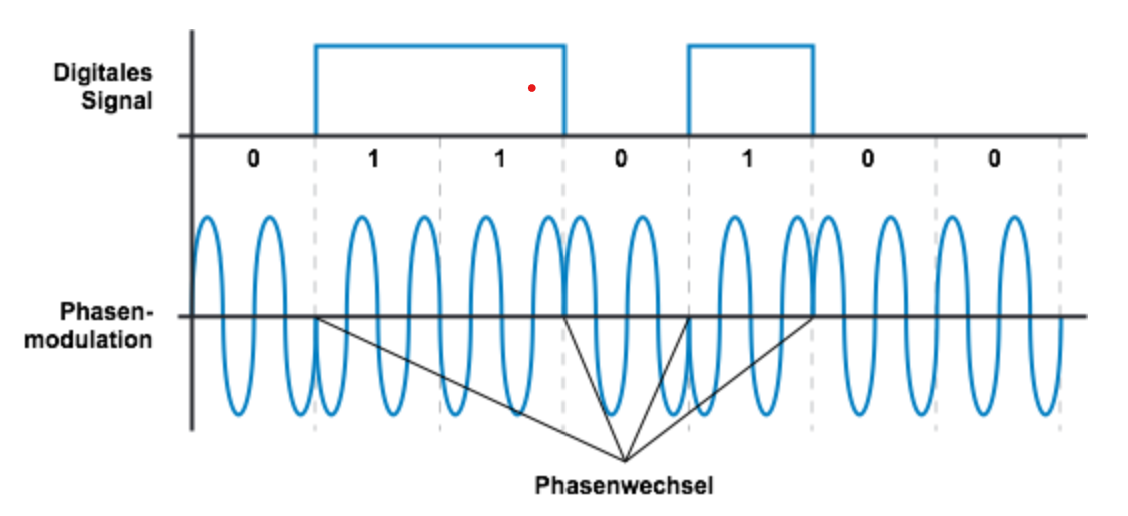
\includegraphics[width=0.5\textwidth]{Pictures/04020211.png}
    \caption{Phasenmodulation}
    \footnotesize{Quelle: \url{https://www.elektronik-kompendium.de/sites/kom/0402021.htm}}
\end{figure}

\section{Blockdiagramm einer Sendestrecke}
Im folgenden Abschnitt wird die Hochfrequenz-Übertragungsstrecke eines typischen Funksystems beschrieben. Bei Abbildung 2.3 handelt es sich um ein Blockdiagramm. Es zielt darauf ab, ein grundlegendes
systematisches Verständnis aufzubauen, um das Gelernte auf unsere spezifische Hardware anwenden zu können. Die einzelnen Komponenten der Hochfrequenz-Übertragungsstrecke
und deren Zusammenspiel werden im Anschluss näher erläutert und auf ihre Realisierung in unserer Hardware eingegangen.\\

\begin{figure}[h]
    \centering
    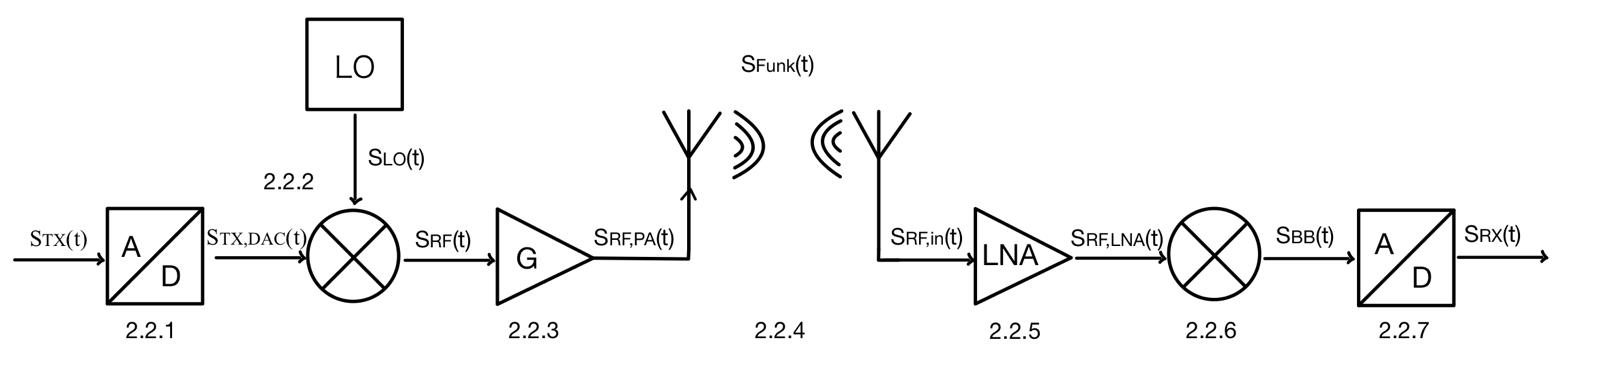
\includegraphics[width=1\textwidth]{Pictures/Blockdiagramm.jpg}   
    \caption{Blockdiagramm einer typischen Hochfrequenz-Übertragungsstrecke}
    %\footnotesize{Quelle: \url{https://www.elektronik-kompendium.de/sites/kom/0402021.htm}}
\end{figure}
\clearpage

\begin{minipage}[t]{0.48\textwidth}
    \raggedright
    \textbf{\large Blockdiagramm-Komponente}\\[2ex]
    \begin{enumerate}
        \item [2.2.1] Digital-Analog-Wandler (DAC)
        \item [2.2.2] Lokaler Oszillator (LO)
        \item [2.2.2] Mischer: Modulator
        \item [2.2.3] Leistungsverstärker (PA)
        \item [2.2.4] Sende- und Empfangsantenne
        \item [2.2.5] Low Noise Amplifier (LNA)
        \item [2.2.6] Mischer: Demodulator
        \item [2.2.7] Analog-Digital-Wandler (ADC)
        
    \end{enumerate}
\end{minipage}%
\hfill
\begin{minipage}[t]{0.48\textwidth}
    \raggedright
    \textbf{\large Beschreibung}\\[2ex]
    \begin{itemize}
        \item $S_{\mathrm{TX}}(t)$: Digital erzeugtes Sendesignal
        \item $S_{\mathrm{TX,DAC}}(t)$: Analoges Signal (Basisbandsignal)
        \item $S_{\mathrm{LO}}(t)$: Sinusförmiges Trägersignal/ ungedämpfte hochfrequente Trägerschwingung
        \item $S_{\mathrm{RF}}(t)$: moduliertes analoges Hochfrequenzsignal
        \item $S_{\mathrm{RF,PA}}(t)$: Verstärkte Hochfrequenzsignal (durch PA)
        \item $S_{\mathrm{Funk}}(t)$: Signal auf Funkstrecke
        \item $S_{\mathrm{RF,in}}(t)$: Schwaches, empfangene Hochfrequenzsignal
        \item $S_{\mathrm{RF,LNA}}(t)$: Verstärkte Hochfrequenzsignal (durch LNA)
        \item $S_{\mathrm{BB}}(t)$: Demoduliertes analoges Basisbandsignal
        \item $S_{\mathrm{RX}}(t)$: Digitalisiertes Basisbandsignal
    \end{itemize}
\end{minipage}



\subsection{DAC}
Ein Digital-Analog-Wandler (eng. digital-to-analog converter, DAC) wandelt digitale Signale oder einzelne Werte in analoge
Signale um. Bei einem digitalen Signal handelt es sich um ein zeitkontinuierliches und wertdiskretes Signal. Durch die Wandlung
in ein analoges Signal wird das Signal zeit- und wertkontinuierlich.  Dafür werden die Rechtecksignale des digitalen Eingangssignals mit Hilfe einer Fouriertransformation
in eine  kontinuierlich veränderliche Spannung transformiert. Diese Wandlung ist erforderlich um das Signal über eine
Antenne aussenden zu können, da Antennen nur elektromagnetische Wellen abstrahlen können. \\
\[S_{TX}(t) \rightarrow S_{TX,DAC}(t)\]
\\

\subsection{LO und Mischer}
Der lokale Oszillator (eng. local oscillator, LO) erzeugt eine ungedämpfte hochfrequente Trägerschwingung. Diese Trägerschwingung
wird benötigt, um das analoge Signal auf die gewünschte Frequenz zu bringen. Der LO kann in verschiedenen Frequenzen arbeiten,
abhängig von der Anwendung und dem gewünschten Frequenzbereich des Signals. In unserer Schaltung ist der LO ein Quarz-Oszillator der bei einer Frequenz $f=1,25GHz$ schwingt.
\\
Schaut man sich den Schaltplan an, so stellt man fest dass folgendes Bauteil der Mischer und LO ist:
\begin{figure}[H]
    \centering
    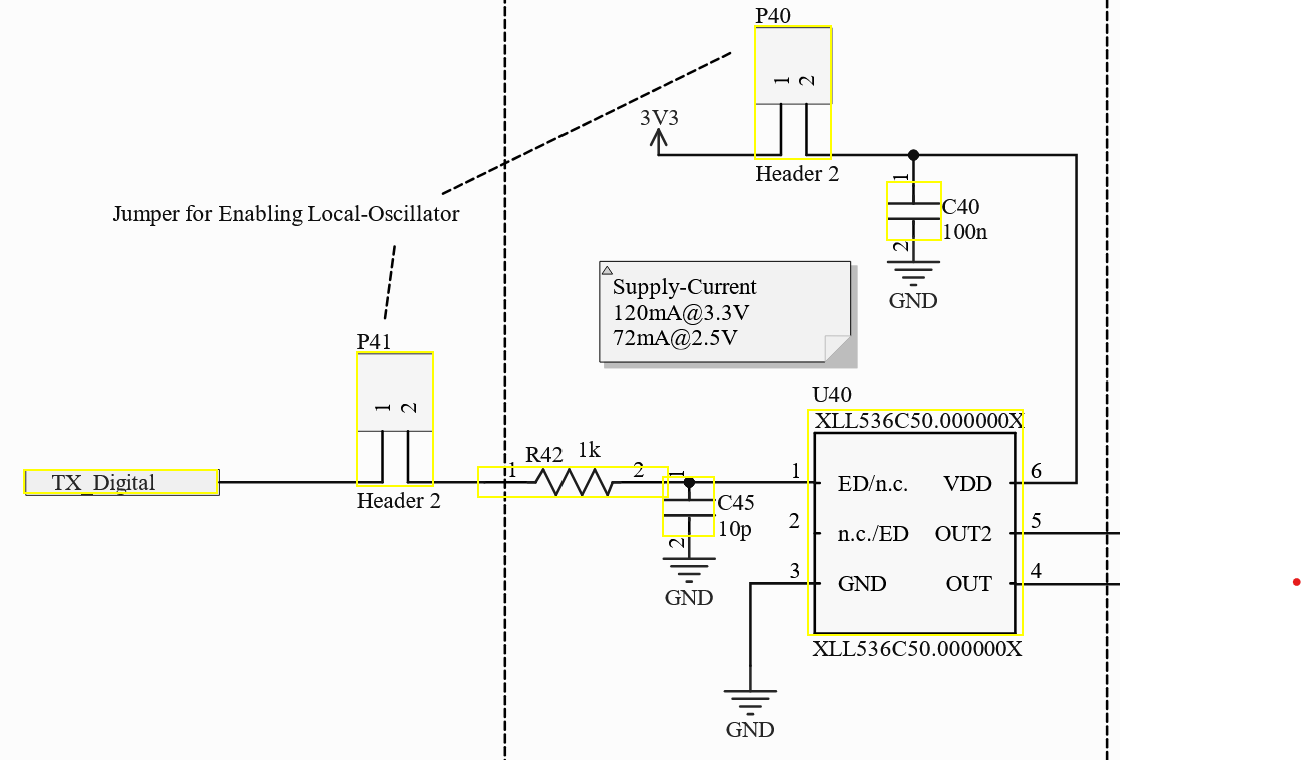
\includegraphics[width=0.8\textwidth]{Pictures/MischerLO.png}
    \caption{Mischer und LO}
    \footnotesize{Quelle: \url{Schaltplan_PCB_V4}}
    \label{fig:link_budget}
\end{figure}
Das digitale Datensignal $TX_{Digital}$ ($D_{TX}$) ist am Oszillator am ED-Eingang angeschlossen.
Ein Blick ins Datenblatt verrät, dass ED der Enable/Disable-Pin ist.
Das bedeutet, der lokale Oszillator wird mithilfe des digitalen Signals an- und ausgeschaltet.
Somit haben wir es mit einer \textbf{digitalen Amplitudenmodulation} zu tun, genauer gesagt mit dem
On-Off-Keying. Das resultierende Signal wird beschrieben durch:

\[S_{TX,DAC}(t)*S_{LO}(t) \rightarrow S_{RF}(t)\]




\subsection{PA}
Der Leistungsverstärker (engl. power amplifier, PA) verstärkt das modulierte Signal auf eine Leistung, die für die Übertragung über eine Antenne 
geeignet ist. Die hohe Leistung ist notwendig, um über eine größere Distanz senden zu können und um Zuverlässigkeit und
Signalqualität zu gewährleisten. 
\[S_{RF}(t) \rightarrow S_{RF,PA}(t)\]

\subsection{Drahtlose Übertragung mit Antennen}
Die Sendeantenne strahlt das modulierte HF-Signal $S_{Funk}$ als elektromagnetische Wellen in den Raum ab. Diese abgestrahlte Welle
breitet sich mit Lichtgeschwindigkeit aus und kann von Empfängerantennen empfangen werden. Die Empfängerantenne wandelt
die elektromagnetische Welle wieder in eine elektrische Spannung um, die dann weiterverarbeitet werden kann. Diese entspricht
jedoch nicht mehr dem ursprünglichen Bandsignal, da es durch Übertragungseinflüsse wie Dämpfung, Rauschen und Interferenzen
und viele weitere Einflüsse gedämpft und gestört wurde.
\[S_{RF,PA}(t) \rightarrow S_{Funk}(t) \rightarrow S_{RF,in}(t)\]

\subsection{LNA}
Bei dem LNA (engl. low noise amplifier) handelt es sich um einen rauscharmen HF-Verstärker. Das empfangene Signal $S_{RF,in}$ ist
durch die bereits erwähnten Einflüsse sehr schwach und muss zuerst verstärkt werden, um weiterverarbeitet werden zu können. Daher
ist eine Verstärkung des Signals unmittelbar nach den Antennen zwingend notwendig. Der Vorteil des LNA gegenüber
anderen Verstärkern ist, dass er kein nennenswertes Rauschen hinzufügt. Dies ist wichtig, da jedes zusätzliche Rauschen
die folgende Demodulation erheblich erschweren würde. Ebenfalls ist durch die Position des LNA das empfangene Signal noch
nicht durch andere elektrische Komponenten verfälscht worden. Wäre dies nicht der Fall, könnte es durch die spätere Verstärkung zu
Rekonstruktionsproblemen des eigentlichen Signals führen.
\begin{figure}[H]
    \centering
    \includegraphics[width=0.4\textwidth]{Pictures/Vorverstärker.jpg}
    \caption{HF-Vorverstärker}
    \footnotesize{Quelle: \url{Schaltplan_PCB_V4}}
    %\label{fig:link_budget}
\end{figure}


Beginnen wir nun die Konversion (=Frequenzumsetzung) vom HF-Signal in ein digitales Nutzsignal im Empfänger in unserer Schaltung. In Abbildung 2.5
wird das empfangene Signal $S_{RF,in}(t)$ über den Kondensator C20 eingekoppelt. Q22 ist hierbei ein HF-Transistorverstärker.\\
\[
S_{RF,in}(t) \rightarrow S_{RF,LNA}(t)
\]
\subsection{Demodulation}
Die Demodulation ist der Prozess, bei dem das modulierte Signal wieder in das ursprüngliche Datensignal zurückgewandelt wird. Dieser Schritt erfolgt
vor dem ADC, weil die Frequenz des Hochfrequenzsignals zu hoch ist, um es direkt mit einem üblichen ADC zu digitalisieren. Die dafür notwendige
Abtastrate wäre hierbei extrem hoch.
Das Nyquist-Abtasttheorem besagt, dass ein Signal der maximalen Frequenz $f_\mathrm{max}$ nur dann verlustfrei rekonstruiert werden kann,
wenn die Abtastfrequenz $f_\mathrm{s}$ mindestens doppelt so groß ist wie $f_\mathrm{max}$:
\begin{equation}
    f_\mathrm{s} \geq 2 f_\mathrm{max}
\end{equation}
Die Trägerfrequenz unseres Modulators beträgt $f=1{,}25\,\mathrm{GHz}$. Das würde eine Abtastrate $f_{s} \geq 2{,}5\,\mathrm{GS/s}$ (S = Samples) erfordern. ADCs, die in der Lage sind, solch hohe Frequenzen
zu verarbeiten, sind kosten-, energie- und datenintensiv. 
\\ 
\begin{figure}[H]
    \centering
    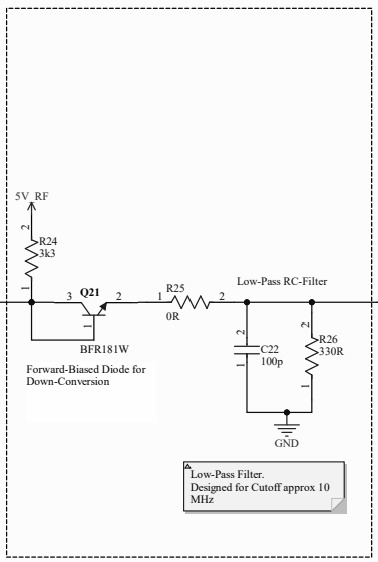
\includegraphics[width=0.4\textwidth]{Pictures/Demodulator.jpg}
    \caption{Demodulator}
    \footnotesize{Quelle: \url{Schaltplan_PCB_V4}}
    %\label{fig:link_budget}
\end{figure}



Die Abbildung 2.6 stellt den Demodulator dar. Der Transistor Q21 ist in Diodenschaltung betrieben. Dadurch werden nur positive Halbwellen des Signals 
durchgelassen (=Gleichrichtung). Danach folgt ein Tiefpassfilter (bestehend aus einer Parallelschaltung aus R26 und C22) mit einer 10-MHz-Grenzfrequenz,
der die hochfrequente Trägerwelle unterdrückt und nur das Basisbandsignal $S_{BB}(t)$ (modulierte Hüllkurve) durchlässt.
\[
S_{RF,LNA}(t) \rightarrow S_{BB}(t)
\]



\subsection{ADC}
Nun muss das demodulierte Signal wieder in ein digitales Signal umgewandelt werden, damit es weiterverarbeitet werden kann.
Der Analog-Digital-Wandler (engl. analog-to-digital converter, ADC) besteht in unserer Schaltung aus zwei Komponenten: einem Analogverstärker und 
einem Komparator.

\begin{figure}[H]
    \centering
    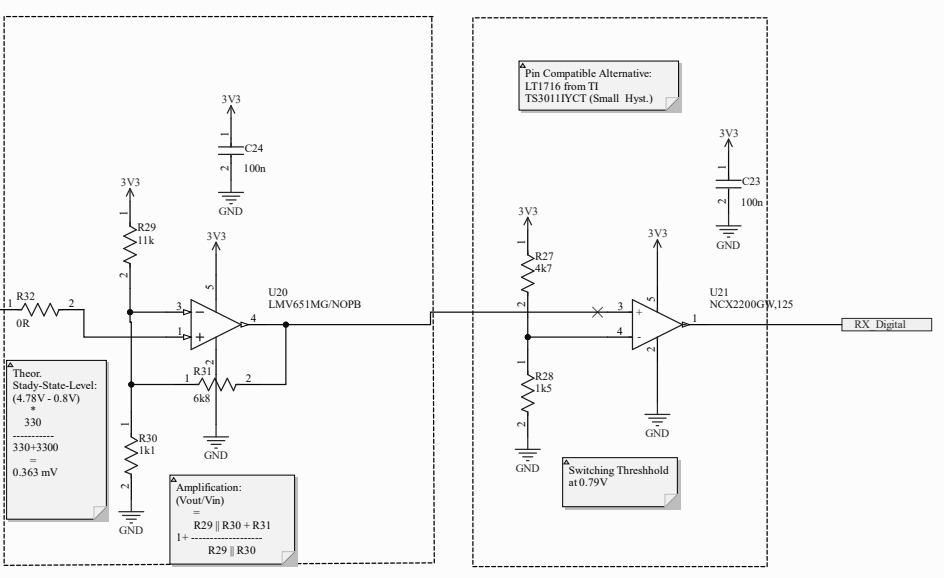
\includegraphics[width=0.8\textwidth]{Pictures/ADC.jpg}
    \caption{Analogverstärker und Komperator}
    \footnotesize{Quelle: \url{Schaltplan_PCB_V4}}
    %\label{fig:link_budget}
\end{figure}

\subsubsection{Analogverstärker}
Der linke Teil der in Abbildung 2.7 dargestellten Schaltung ist der Analogverstärker. Das geschwächte analoge Signal durchläuft den 
Operationsverstärker U20, um den Pegel oberhalb des festgelegten Schwellwerts für die Komparatorschaltung zu bringen.


\subsubsection{Komparator}
Die rechte Seite der Schaltung bildet der Komparator U21. Dieser vergleicht das demodulierte Signal $S_{BB}(t)$ mit einem festen Schwellwert von 0,79 V.
Wird dieser Schwellwert überschritten, gilt:
\[
S_{BB}(t) > 0{,}79\,\mathrm{V} \implies \text{HIGH}
\]
\[
S_{BB}(t) < 0{,}79\,\mathrm{V} \implies \text{LOW}
\]
Dadurch wird ein binäres digitales Ausgangssignal erzeugt, das von einem Computer weiterverarbeitet werden kann.
\[
S_{BB}(t) \rightarrow S_{RX}(t)
\]

\clearpage

\section{Mathematische Grundlagen: Fourier-Transformation}
Übersichtlichkeitshalber werden in diesem Abschnitt für die Fourier-Transformation die Werte $w_0 = 4\pi$ für Sinusfunktion und $T = 2$ für Rechteckfunktion angenommen. Dies ändert jedoch im Allgemeinen nichts an der Theorie, sondern vereinfacht lediglich die Darstellung der Grafiken.
\subsection{Betrag und zeitlicher Verlauf von Rechteckfunktion}
Der Rechteckimpuls ist eine wichtige Funktion in der Signalverarbeitung.
Er wird häufig in der Kommunikationstechnik verwendet, um digitale Signale zu repräsentieren.
Der Verlauf der Rechteckfunktion $x(t)$ ist in Abbildung \ref{fig:rechteck} dargestellt.
\begin{figure}[H]
    \centering
    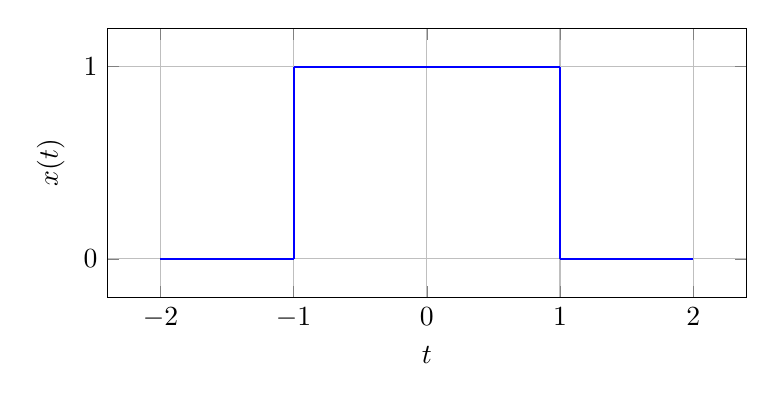
\begin{tikzpicture}
        \begin{axis} [
            width=0.8\textwidth,
            height=5cm,
            axis lines=box, % Rahmen um den Plot
            xlabel={$t$},
            ylabel={$x(t)$},
            domain=-2:2,
            samples=200,
            xtick={-2,-1,0,1,2},
            ytick={0,1},
            ymin=-0.2, ymax=1.2,
            grid=both,
        ]
        % Null-Linie links
        \addplot[blue, thick, samples=2, domain=-2:-1] {0};
        % Rechteck oben
        \addplot[blue, thick, samples=2, domain=-1:1] {1};
        % Null-Linie rechts
        \addplot[blue, thick, samples=2, domain=1:2] {0};
        % Vertikale Linie bei t=-1
        \addplot[blue, thick, samples=2, domain=0:1] ({-1},{x});
        % Vertikale Linie bei t=1
        \addplot[blue, thick, samples=2, domain=0:1] ({1},{x});
        \end{axis}
    \end{tikzpicture}
    \caption{Verlauf der Rechteckfunktion $x(t)$ mit Amplitude 1 im Intervall $-1 < t < 1$}
    \label{fig:rechteck}
\end{figure}

Die Rechteckfunktion $x(t)$ ist gegeben durch:
\[
x(t) = \begin{cases}
    1 & \text{für } -1 < t < 1 \\
    0 & \text{sonst}
    \end{cases}
\]
    
Die Fourier-Transformierte einer Rechteckfunktion der Breite $2T$ und Höhe $1$ ist gegeben durch die normierte $\mathrm{sinc}$-Funktion:
\[
\mathcal{F}\{x(t)\} = 2T \cdot \mathrm{sinc}(T\omega) = 2T \cdot \frac{\sin(T\omega)}{T\omega}
\]
\clearpage
Der Verlauf der Fourier-Transformierten ist in folgender Abbildung dargestellt:

\begin{figure}[h]
    \centering
    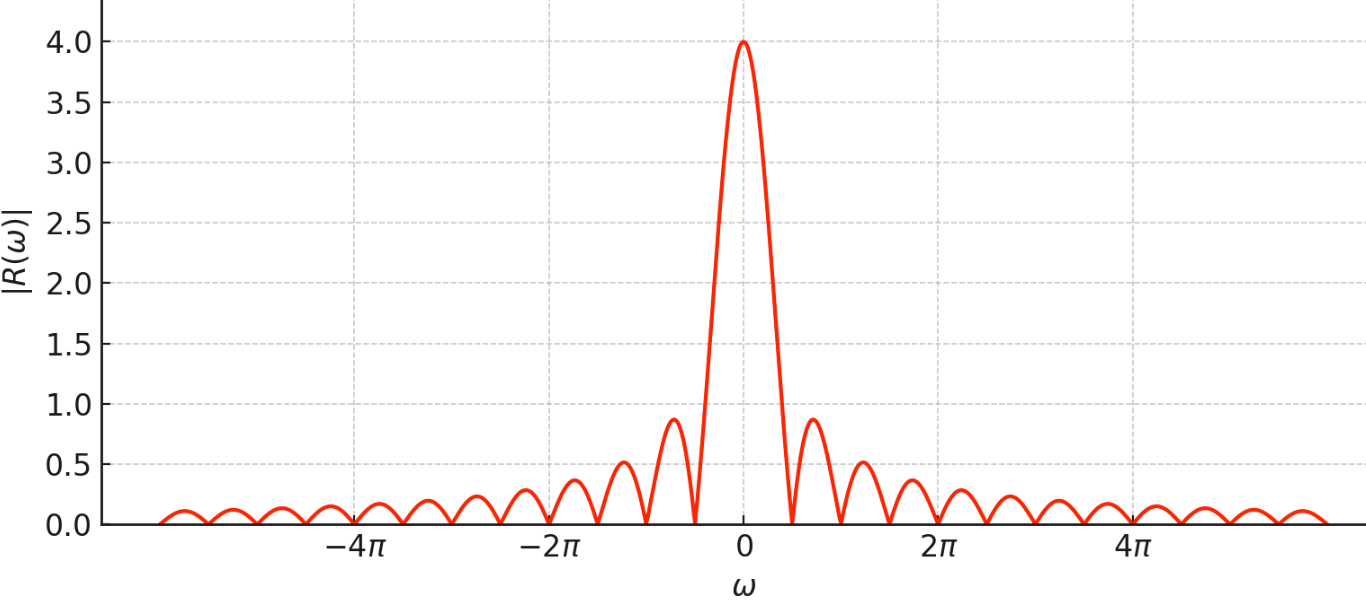
\includegraphics[width=0.8\textwidth]{Pictures/rechteckFourier.png}
\caption{Betragsspektrum eines Rechteckpulses der Breite $T = 2$}
\label{fig:fourier_rechteck}
\end{figure}

Die Rechteckfunktion ist in der digitalen Signalverarbeitung von Relevanz, da sie eine Basis für die Änderung des Signalpegels darstellt. Durch die Idealisierung lässt sich der High-Pegel (1) und Low-Pegel (0) des Signals gut darstellen. In der Praxis wird die Rechteckfunktion durch eine $\mathrm{sinc}$-Funktion approximiert, um Übertragungsfehler zu minimieren.

\subsection{Betrag und zeitlicher Verlauf von Sinusfunktion}
Der Sinus ist eine wichtige Funktion in der Signalverarbeitung.
Er beschreibt eine harmonische Schwingung und ist in der Fourier-Analyse von Bedeutung. Sein Verlauf ist in der Abbildung \ref{fig:sinus} dargestellt.
Die Sinusfunktion $x(t) = \sin(t)$ hat eine Periode von $2\pi$ und schwingt zwischen -1 und 1. Sie ist punktsymmetrisch um den Koordinatenursprung, was bedeutet, dass $x(-t) = -x(t)$ gilt. Dies ist eine Eigenschaft der ungeraden Funktion.

\begin{figure}[H]
\centering
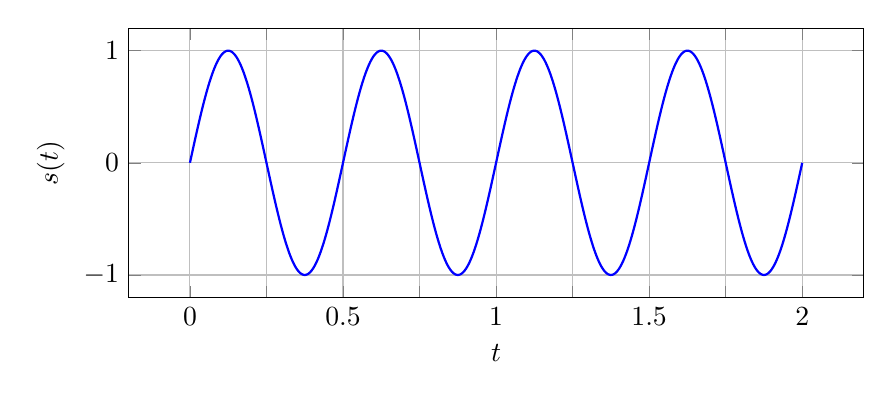
\begin{tikzpicture}
\begin{axis}[
    width=0.9\textwidth,
    height=5cm,
    xlabel={$t$},
    ylabel={$s(t)$},
    domain=0:2,
    samples=500,
    grid=major,
    xtick={0, 0.25, 0.5, 0.75, 1, 1.25, 1.5, 1.75, 2},
    xticklabels={$0$, , $0.5$, , $1$, , $1.5$, , $2$},
    ymin=-1.2, ymax=1.2,
    declare function={
        omegaNull = 4*pi;
    },
]
\addplot[blue, thick] {sin(deg(omegaNull * x))};
\end{axis}
\end{tikzpicture}
\caption{Zeitverlauf des Sinussignals $s(t) = \sin(\omega_0 t)$ mit $\omega_0 = 4\pi$}
\label{fig:sinus}
\end{figure}



Die Fourier-Transformierte der Sinusfunktion $x(t) = \sin(t)$ ist gegeben durch:
\[
\mathcal{F}\{\sin(\omega_0 t)\} = \pi j \left[ \delta(\omega + \omega_0) + \delta(\omega - \omega_0) \right]
\]

Der Betrag der Fourier-Transformierten besteht also aus zwei Dirac-Impulsen bei $\omega = \pm \omega_0$.

Die graphische Darstellung der Fourier-Transformierten der Sinusfunktion ist in Abbildung \ref{fig:fourier_sinus_komplex} zu sehen.
\begin{figure}[H]
\centering
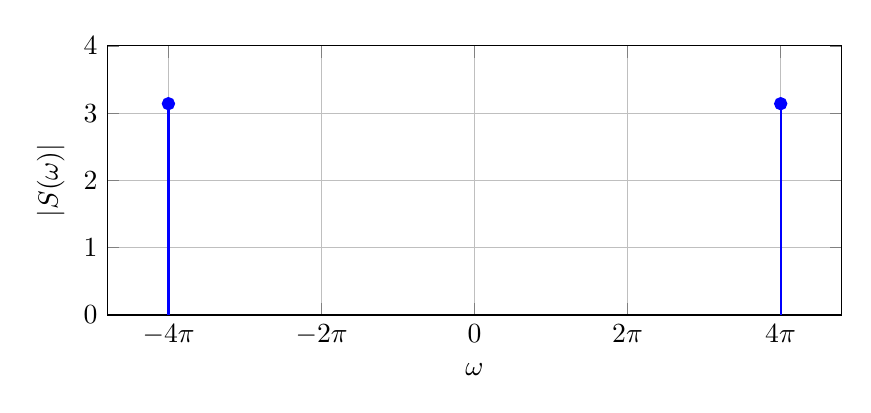
\begin{tikzpicture}
\begin{axis}[
    width=0.9\textwidth,
    height=5cm,
    xlabel={$\omega$},
    ylabel={$|S(\omega)|$},
    domain=-15:15,
    samples=1000,
    ymin=0, ymax=4,
    xtick={-12.56, -6.28, 0, 6.28, 12.56},
    xticklabels={$-4\pi$, $-2\pi$, $0$, $2\pi$, $4\pi$},
    grid=major,
]
\addplot[blue, ycomb, thick, mark=*] coordinates {(-4*pi, 3.14) (4*pi, 3.14)};
\end{axis}
\end{tikzpicture}
\caption{Betragsspektrum eines Sinussignals $s(t) = \sin(\omega_0 t)$ mit $\omega_0 = 4\pi$}
\label{fig:fourier_sinus_komplex}
\end{figure}

Die Sinusfunktion spielt eine immens wichtige Rolle in der digitalen Signalverarbeitung, da sie der Grundstein der Fourier-Analyse (Fourier-Reihen und Fourier-Transformation) ist. Auch sind diese für lineare zeitinvariante Systeme (LTI) von Bedeutung. 
Der Sinus ist eine elementare periodische Funktion, seine Periodizität ist das grundlegende Konzept in vielen Signalen. Er lässt auch unter anderem komplex erscheinende Funktionen in Sinuskomponenten zerlegen und somit sie einfacher und kompakter darstellen.
Auch in der analogen Signalverarbeitung ist der Sinus von Bedeutung, da er die Basis für die Amplituden-, Frequenz- und Phasenmodulation bildet. Schließlich ist die Idealform der aus der Steckdose kommenden Netzspannung eine Sinuswelle, die in vielen Anwendungen als Referenzsignal dient. 

\subsection{Multiplikation der beiden Funktionen im Zeitbereich}
Bei einer Multiplikation der beiden Funktionen im Zeitbereich, also der Rechteckfunktion $x(t)$ und der Sinusfunktion $y(t)$, ergibt sich eine neue Funktion $z(t) =  x(t) \cdot y(t)$, die in Abbildung \ref{fig:rechteck_sinus} dargestellt ist. Diese Funktion ist das Ergebnis der Punkt-für-Punkt-Multiplikation der beiden Funktionen.

\begin{figure}[H]
    \centering
    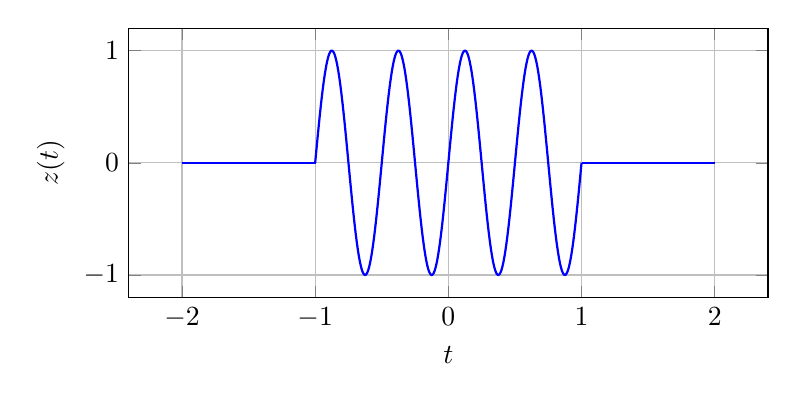
\begin{tikzpicture}
        \begin{axis}[
            width=0.8\textwidth,
            height=5cm,
            axis lines=box,
            xlabel={$t$},
            ylabel={$z(t)$},
            domain=-2:2,
            samples=500,
            xtick={-2,-1,0,1,2},
            ytick={-1,0,1},
            ymin=-1.2, ymax=1.2,
            grid=both,
        ]
            % Rechteckfunktion * Sinus im Intervall -1 < t < 1
            \addplot [
                thick,
                blue,
                domain=-1:1
            ] {sin(deg(4*pi*x))};
            % Null außerhalb des Rechtecks
            \addplot[
                thick,
                blue,
                domain=-2:-1
            ] {0};
            \addplot[
                thick,
                blue,
                domain=1:2
            ] {0};
        \end{axis}
    \end{tikzpicture}
    \caption{Multiplikation der Rechteckfunktion $x(t)$ (Breite $T=2$) mit der Sinusfunktion $y(t) = \sin(4\pi t)$}
    \label{fig:rechteck_sinus}
\end{figure}

Die Fourier-Transformierte der Multiplikation zweier Funktionen im Zeitbereich ist gegeben durch die Faltung ihrer Fourier-Transformierten im Frequenzbereich. Das bedeutet, dass die Fourier-Transformierte von $z(t)$, also $\mathcal{F}\{z(t)\}$, das Ergebnis der Faltung der Fourier-Transformierten von $x(t)$ und $y(t)$ ist:
\[
\mathcal{F}\{z(t)\} = \mathcal{F}\{x(t)\} * \mathcal{F}\{y(t)\}
\]

Die analytische Form der Funktion aus dem Bild lautet:
\[
\left| \mathcal{F}\{z(t)\} \right| = \left| \frac{T}{2} \left( 
\operatorname{sinc}\left(\frac{(\omega-\omega_0)T}{2\pi}\right)
+ 
\operatorname{sinc}\left(\frac{(\omega+\omega_0)T}{2\pi}\right)
\right) \right|
\]

% Plot der Funktion mit Beispielwerten T=2, \omega_0=4\pi
\begin{figure}[h]
\centering
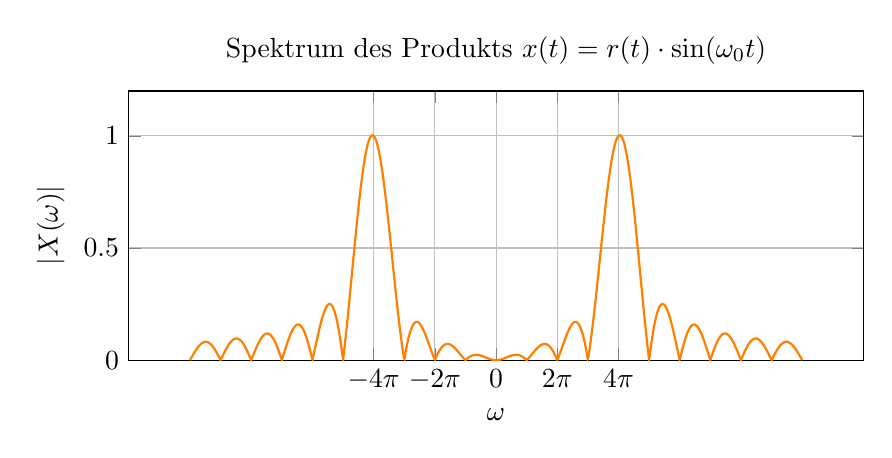
\begin{tikzpicture}
\begin{axis}[
    width=0.9\textwidth,
    height=5cm,
    xlabel={$\omega$},
    ylabel={$|X(\omega)|$},
    title={Spektrum des Produkts $x(t) = r(t) \cdot \sin(\omega_0 t)$},
    domain=-10*pi:10*pi,
    samples=1000,
    ymin=0, ymax=1.2,
    xtick={-12.56, -6.28, 0, 6.28, 12.56},
    xticklabels={$-4\pi$, $-2\pi$, $0$, $2\pi$, $4\pi$},
    grid=major,
    declare function={
        T = 2;
        omegaNull = 4*pi; % du kannst das später in der Präambel als \def\omegaNull{4*pi} setzen
        sinc(\x) = (abs(\x) < 1e-3) ? 1 : sin(deg(\x))/\x;
    },
]
\addplot[orange, thick, domain=-10*pi:10*pi] 
    {abs( (T/2)*(sinc((x - omegaNull)*T/2) + sinc((x + omegaNull)*T/2)) )};
\end{axis}
\end{tikzpicture}
\caption{Allgemeines Betragsspektrum $|X(\omega)|$ des Produkts mit variabler Frequenz $\omega_0$ und Rechteckbreite $T$}
\label{fig:fourier_rechteck_sinus}
\end{figure}


Somit ergibt sich eine Faltung der beiden $\mathrm{sinc}$-Funktionen, die in Abbildung \ref{fig:fourier_rechteck_sinus} dargestellt ist. Diese Faltung führt zu einem Frequenzspektrum, das die Eigenschaften beider Funktionen kombiniert.
\clearpage